\documentclass{article}

\usepackage{fancyhdr}
\usepackage{cmap}
\usepackage[T2A]{fontenc}
\usepackage[utf8]{inputenc}
\usepackage[english,russian,ukrainian]{babel}
\usepackage{indentfirst}
\usepackage{graphicx}
\usepackage{hyperref}
\usepackage{titlesec}
\usepackage{fancyhdr}
\usepackage{geometry}
\usepackage{titlesec}
\usepackage{scrextend}

\hypersetup{
	colorlinks,
	citecolor=black,
	linkcolor=black,
	filecolor=black,
	urlcolor=black
}

\geometry{
	a4paper,
	total={165mm,247mm},
	left=20mm,
	top=30mm,
}

\pagestyle{fancy}
\fancyhf{}
\renewcommand{\headrulewidth}{0.5pt}
%\renewcommand{\footrulewidth}{0.1pt}
\rhead{\LaTeX}
\lhead{Вячеслав Козачок}

\cfoot{\thepage}
%\titleformat{\section}
%{\normalfont\Large\bfseries}{\thesection}{1em}{}

%\titleformat*{\subsection}{\large\bfseries}

 \usepackage{listings}
 \usepackage{xcolor}
 
 \definecolor{codegreen}{rgb}{0,0.6,0}
 \definecolor{codegray}{rgb}{0.5,0.5,0.5}
 \definecolor{codepurple}{rgb}{0.58,0,0.82}
 \definecolor{backcolour}{rgb}{0.99,0.99,0.99}
 \definecolor{codeblue}{rgb}{0.1,0.1,0.99}
 
 \lstdefinestyle{mystyle}{
 	backgroundcolor=\color{backcolour},   
 	commentstyle=\color{codegreen},
 	keywordstyle=\color{codeblue},
 	numberstyle=\tiny\color{codegray},
 	stringstyle=\color{codepurple},
 	basicstyle=\ttfamily\footnotesize,
 	breakatwhitespace=false,         
 	breaklines=true,                 
 	captionpos=b,                    
 	keepspaces=true,                 
 	numbers=left,                    
 	numbersep=5pt,                  
 	showspaces=false,                
 	showstringspaces=false,
 	showtabs=false,                  
 	tabsize=4
 }
 
 \lstset{style=mystyle}
 
 
\begin{document}
 \begin{titlepage}
	
	\begin{frame}[t]
		\raisebox{-10mm}[10pt][0pt]{%
			\makebox[\textwidth][c]{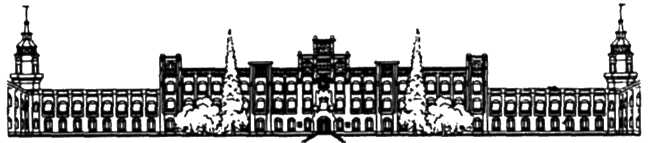
\includegraphics[width=\textwidth]{institute.jpg}}
		}
	\end{frame}\\
	\large
	\centering{
		\vspace{5mm}\\
		Міністерство освіти і науки України \\
		Національний технічний університет України \\
		``Київський політехнічний інститут імені Ігоря Сікорського''\\
		Фізико-технічний інститут
	}
	\vspace{3cm}\\
	\centering{
		{\Huge\textbf{Криптографія} \\ \vspace{0.2cm}}
		{\huge Лабораторна №1}
	}
	
	\vspace{8cm}
	\Large
	\begin{flushright}
		Виконали:\\
		Студенти групи ФБ-82\\
		\textbf{Козачок Вячеслав \\ Ілля Кузнєцов}\\
		Перевірив: \\
		
	\end{flushright}
	\vfill
	
	\centering{Київ - 2020}
	
\end{titlepage}
 \newpage
 \large
 \section{Порядок виконання роботи}
\begin{enumerate}
	\item Уважно прочитати методичні вказівки до виконання комп’ютерного практикуму.
	\item Написати програми для підрахунку частот букв і частот біграм в тексті, а також підрахунку H1 та H2 за безпосереднім означенням. Підрахувати частоти букв та біграм, а також значення H1 та H2 на довільно обраному тексті російською мовою достатньої довжини (щонайменше 1Мб), де імовірності замінити відповідними частотами. Також одержати значення H1 та H2 на тому ж тексті, в якому вилучено всі пробіли.
	\item За допомогою програми CoolPinkProgram оцінити значення H(10), H(20), H(30) 
	\item Використовуючи отримані значення ентропії, оцінити надлишковість російської
	мови в різних моделях джерела.
\end{enumerate}

\section{Методичні вказівки}
Звичайні текстові файли містять багато символів окрім власне літер; для обчислення значень ентропій вони повинні пройти попередню фільтрацію: всі символи, окрім текстових, повинні вилучатись або замінюватись на пробіли; прописні літери - замінюватись на відповідні стрічні; послідовність пробілів (або інших розділових знаків, наприклад, символів кінця рядку) повинна трактуватись як один пробіл або вилучатись, якщо пробіл не входить до алфавіту.


При підрахунку частот біграм треба розглядати як пари букв, що перетинаються, так і пари букв, що не перетинаються (тобто рухатися вздовж тексту з кроком 2). Одержані результати не повинні суттєво відрізнятись, однак в першому випадку використовується більше статистики, а тому чисельні дані більш точні. Таблицю частот символів потрібно подавати відсортованою за спаданням частот. Таблицю частот біграм зручно подавати у вигляді квадратної матриці, індексованої першою та другою літерами біграм.
	
	
Програма CoolPinkProgram використовує текст, що лежить у допоміжному файлі text. Цей текст написаний російською мовою без знаків пунктуації та великих літер; буква «ё» замінена буквою «е», а «ъ» – буквою «ь». Пробіл також вважається буквою. Таким чином, кількість букв алфавіту m=32. При підрахунку H(10), H(20), H(30) виконати не менш ніж 50 експериментів.


\newpage
\section{Частота}

\normalsize
\begin{minipage}[t]{.5\textwidth}
	\begin{verbatim}
	а:  117081
	б:   24717
	в:   66549
	г:   25689
	д:   41627
	е:  123629
	ж:   16018
	з:   23117
	и:   93860
	й:   14860
	к:   48456
	л:   70907
	м:   40517
	н:   98121
	о:  162385
	п:   34091
	р:   56282
	\end{verbatim}
\end{minipage}% <---------------- Note the use of "%"
\begin{minipage}[t]{.5\textwidth}
\begin{verbatim}
	с:   75105
	т:   84627
	у:   38126
	ф:    1779
	х:   10981
	ц:    3992
	ч:   23851
	ш:   12067
	щ:    4054
	ъ:     412
	ы:   26210
	ь:   27849
	э:    5018
	ю:    8811
	я:   30439
	ё:      31
\end{verbatim}
\end{minipage}

\section{Відсортовано за кількістю літер}
\begin{minipage}[t]{.5\textwidth}
	\begin{verbatim}
о:  162385
е:  123629
а:  117081
н:   98121
и:   93860
т:   84627
с:   75105
л:   70907
в:   66549
р:   56282
к:   48456
д:   41627
м:   40517
у:   38126
п:   34091
я:   30439
ь:   27849
	\end{verbatim}
\end{minipage}% <---------------- Note the use of "%"
\begin{minipage}[t]{.5\textwidth}
	\begin{verbatim}
ы:   26210
г:   25689
б:   24717
ч:   23851
з:   23117
ж:   16018
й:   14860
ш:   12067
х:   10981
ю:    8811
э:    5018
щ:    4054
ц:    3992
ф:    1779
ъ:     412
ё:      31
	\end{verbatim}
\end{minipage}

\newpage
\section{Биграмы}
\tiny
\begin{addmargin}{-4em}
 \begin{verbatim}
     а     б     в     г     д     е     ж     з     и     й     к     л     м     н     о     п     р     с     т     у     ф     х     ц     ч     ш     щ     ъ     ы     ь     э     ю     я     ё    
а     11   991  5118   984  3639  1723  1881  6997   212   885  6997 16127  4035  7743    11   995  3933  5895  6974    85   428  1415   202  1312  1067   340     0     0     0    10  1405  4032     0
б   1399     2   143     6    54  3344     9     4  1301     0   400  1330    96   502  3306     0  1837   134    13  1631     0    91    10    10    14   416   187  6943    25     0     8   836     0
в   9176    27    36    51   520  7168     2   892  7585     0   252  1301   241  2121 11764   344  1780  5804   382  1103     0    96    39   129  1781    13     7  4011   315     0     4   438     0
г   1402     1    12     4  1921   599     0     1  1258     0   199  2516     1   289 14057     0  1142    49    11   984     2     0     0    63     9     0     0     0     0     0     6     0     0
д   7080    37  1274     7    62  7549    23     2  3425     0   349  1332   116  2549  6188   108  2475   566   311  3001     0   102   293    45   170     1    97   887  1288     0    12   659     0
е     86  2152  4193  6124  4086  3617  1321  1950   161  4193  2930  9643  6709 12230   322  2253  8757  6448  7475   152    18  1313   269  1503  1552  1019     0     0     0     0   661   590     0
ж   2322    73     0     9  1285  6803    19     0  2447     0   150     6     4  1660    74     0     1   159     0   405     0     0     1    67     0     0     0     0    68     0     2     0     0
з   8939   267  1349   865  1284   397   175    32   506     0   158   308   463  3255   599     0   339    87    22   434     0     0     7    92    11     0    24   637   266     0     7   794     0
и    158   644  4450   697  2582  4046   522  2995  1029  2238  2654  7409  4664  6906   154   233   895  3587  6389    17    23  2190  1366  3146   655   248     0     0     0     1   417  2905     0
й      0     2     0     0   340     2     0     1     0     0   108   144    87   455     3     0     3   832   392     0     7     0    70   118    87     1     0     0     0     0     0     0     0
к  12951     0   281     0     6   839    23     7  4793     0    28   549     1  1023 13138     0  2315  1548   669  2360     2     2    12     0    18     0     0     0     0     0     0     0     0
л  12768    29     6   193    23  8789   630     5  8842     0   473   425     1   483  9707    71     0  2023    41  1986     7     0     1   194     6     1     0  1557  5912     0  1684  2905     3
м   4152    21     6    48     0  4966     1     5  4412     0    88   152    67  2095  5263    94   121   181    32  4573     2     0    16    31     7     8     0  1550   116     0     4   644     0
н  18414    22    13   166  1061 16578     7    23 12993     0   420     0     3  4869 16319     0   142  1769   704  4069    27     2   580   425     2   264     0  4874  2060     0   257  2848     0
о      4  5763 12275  7737  7043  4154  3172  1698  1196  5141  2584  9205  8093 13884   308  1873  9112  9822 10561    86   239   569   149  2680  2065   247     0     0     0    70  1320   831     0
п   1926    12     0     0     0  3515     0     0  1359     0    97   765     0   106 13697    40 10400    13    81   858     1     0    24    52    22     5     0   420    59     0     5   558     0
р  11536   377   507   599   566  8820   502    26  7389     0   939    82   218  1115 11579    97    27   344   767  3785    18   160    47   113   351    51     0  2050  1437     0   184  1474     0
с   2976    87  3044    17   527  7352    43    31  2217     0  8474  4231  1369  1587  4040  2805   203  1014 17645   862    13   225    97   715   102     3    38   550  4691     3   208  5024    27
т   8312    21  4463    10   195  8392     8     3  6403     0   799   430    35  1799 24151    81  4067  1431   134  1942    35    17   101   458     1    21    58  2471 10409     4    76   874     0
у     62   873  1853  1624  2533   428  2858   492     5   199  1252  1881  1950   353     6   952   926  1670  1732     1    30   491     6  1451  1160   328     0     0     0    25  1604   191     0
ф    149     0     0     0     0   204     0     0   519     0     0    41     5     3   163     0   418    18    31    42    12     0     0     1     0     0     0     8    89     0     2     2     0
х   1367     0   159     2     1    59     0     0   188     0     0   143    81   162  3708     1   113    70    10   250     0     0     0     1    15     0     1     0     0     0     0     0     0
ц    784     1    63     0     0  1122     0     0   321     0   185     1     2     0   457     0     0     0     0   349     0     0    12     0     0     0     0   251     0     0     0     0     0
ч   3729     0     7     0     0  5646     0     0  2161     0   517    71     8   814    82     0   100     0  7356  1519     0     0     0     0   279     0     0     0   267     0     0     0     0
ш   1511     0   140     0     0  3775     0     0  2539     0   593   903     8   613   465    10     2     0   106   473     2     0     4     0     2     0     0     0   807     0     6     0     0
щ    485     0     0     0     0  2191     0     0  1114     0     0     0     0    53     2     0     9     0     0   148     0     0     0     0     0     0     0     0    39     0     0     0     0
ъ      0     0     0     0     0   202     0     0     0     0     0     0     0     0     0     0     0     0     0     0     0     0     0     0     0     0     0     0     0     0    12   196     0
ы      0   774  1630   149   223  1590    41   103     9  1995   270  4303  1939   546     0   189   463  1277  1187     9     0  1382     1   292   704     1     0     0     0     0     0     3     0
ь      0   151    48    83    43   811     2   281   681     0  1974     0   360  1969    14     6     0  1369   118     0     4     2   170   100   678    25     0     0     0     4   646   679     0
э      0     0     2     4     3     0     0    10     0     5    66    71     3    40     0    36    12     7  4748     0     3     0     0     0     1     0     0     0     0     0     0     0     0
ю      3  1049     5     6   396     0    11     6     2     0     6    24    27    42     0    14    66   269   417     0     3    16    18    68    42   554     0     0     0     0    57     0     0
я      0    41   431   464   889   127   477   526    64   200   180  1358   537  1109     0    92    77  1407  2259     1     0   314    58   203    79   336     0     0     0     0   166   225     0
ё      0     0     3     0     0     0     0     0     0     0     1     0     0     0     0     0     0     0     0     0     0     0     0     0     0     0     0     0     0     0     0     0     0
 \end{verbatim}
\end{addmargin}

\end{document}